\documentclass[10pt]{article}
\usepackage[a4paper,margin=1.85cm]{geometry}
\usepackage[T1]{fontenc}
\usepackage{lmodern}
\usepackage{microtype}
\usepackage{amsmath}
\usepackage{booktabs}
\usepackage{graphicx}
\usepackage{caption}
\usepackage{float}
\usepackage[hidelinks]{hyperref}
\graphicspath{{figures/}}
\setlength{\parskip}{0.32em}
\setlength{\parindent}{0pt}
\captionsetup{font=small,labelfont=bf,skip=3pt}
\setlength{\textfloatsep}{7pt}
\setlength{\intextsep}{7pt}

\title{\vspace{-1.6em}Performance analysis comparison on two different GPUs}
\author{}
\date{\vspace{-2.4em}}

\begin{document}
\maketitle
\vspace{-1.0em}

\textbf{Summary.} We compare the real-time performance of two emissive-texture light samplers,
BudgetLeafAlias and CodecLeafAlias, against a dense 2D CDF and three further baselines, on two
graphics processors at opposite ends of the same architecture: an NVIDIA RTX 4080 SUPER desktop card
and an NVIDIA RTX 4050 Laptop part. The question is how much of the advantage these techniques hold
over the 2D CDF survives, or changes, when the hardware shrinks. Two studies are reported for both
processors. The first measures how much faster each technique reaches the image quality the 2D CDF
achieves inside a 33.3\,ms real-time frame. The second sweeps the leaf budget of BudgetLeafAlias and
measures what it costs. The headline is that the advantage does not shrink on the smaller part, it
grows: averaged over the three scenes, BudgetLeafAlias is $1.31\times$ faster than the 2D CDF at
equal quality on the 4080 SUPER and $1.94\times$ on the 4050, and CodecLeafAlias $1.38\times$ and
$1.89\times$. Every technique in the comparison gains ground on the 2D CDF on the smaller GPU, so
part of this is the 2D CDF being penalised rather than our techniques improving; but our two gain
the most and keep the largest margin on both processors.

\section*{1\quad Two GPUs}

\begin{table}[H]
\centering\small
\begin{tabular}{lll}
\toprule
& RTX 4080 SUPER & RTX 4050 Laptop \\
\midrule
Architecture & Ada (AD103) & Ada (AD107) \\
Streaming multiprocessors & 80 & 20 \\
L1 cache / shared memory per SM & 128\,kB & 128\,kB \\
L2 cache & 64\,MB & \textbf{24\,MB} \\
Device memory & 16\,GB & 6\,GB \\
Board power & 320\,W & \textbf{35\,W} \\
Host CPU & Core i7-14700F & Core i9-13900H \\
\bottomrule
\end{tabular}
\caption{The two processors. They share the Ada streaming multiprocessor, so the first-level cache
is the same size on both; the smaller part has a quarter of the multiprocessors, roughly a quarter
of the memory interface, 2.7 times less second-level cache and a ninth of the power budget. The
4050's L2 capacity is not a vendor figure but a measurement: a pointer-chase benchmark on this
machine holds a flat 67.7\,ps per dependent read out to a 24\,MB working set and then collapses, to
133.5\,ps at 28\,MB and 409\,ps at 64\,MB. The same benchmark places the first-level limit at
128--192\,KB on both parts.}
\label{tab:gpus}
\end{table}

\emph{The techniques.} All six draw a light sample from an emissive texture on a quad light. The
\emph{2D CDF} inverts a cumulative distribution built over every texel, which costs about 24
dependent memory reads per sample over a table as large as the image. \emph{2D CDF/8} builds the
same structure at one eighth of the resolution. \emph{Mipmap} warps a sample down a mip pyramid.
\emph{Alias per pixel} is an alias table with one entry per texel, $O(1)$ sampling but two dependent
reads spread over a structure of tens of megabytes. \emph{BudgetLeafAlias} partitions the emitter
into a bounded number of leaves, $B$, and runs an alias table over those leaves instead of over
texels; at $B=4000$ its structure is about 75\,KB. \emph{CodecLeafAlias} derives its partition from
the texture's own codec structure. The last two are the techniques under test.

\section*{2\quad How performance is measured}

For each scene and technique we render a ladder: at each of twelve light-sample counts per shading
point, from 1 to the engine's limit of 64, we render forty frames at $1920\times1080$, take the
median frame time after a twelve-frame warm-up, and capture one frame to compare against a converged
reference of the same scene. Illumination is direct only and the quad light is the scene's only
light source, so that the error being measured is the light-sampling error and not residual
path-tracing noise; primary samples are taken at pixel centres for the same reason. The reference is
1200 accumulated frames at the maximum light-sample count. RMSE against that reference is smoothed
by a quadratic fit of $\log(\mathrm{MSE})$ against $\log(\mathrm{samples})$, because a single rung is
noisy.

From the ladder we read two numbers. \emph{Equal quality}: the 2D CDF's frame time is filled to
33.3\,ms, its RMSE there is recorded, and each technique's speed-up is 33.3\,ms divided by the frame
time at which that technique reaches the same RMSE. \emph{Equal time}: each technique's RMSE inside
33.3\,ms, relative to the 2D CDF's.

\emph{Provenance, and where the two columns differ.} The RTX 4050 Laptop numbers throughout this note
are measured on that machine with the protocol just described. The RTX 4080 SUPER equal-quality
numbers are the same measurement, on the same six techniques and the same three scenes, taken from
this project's own equal-quality experiment; that experiment is also direct illumination, but it
integrates RMSE over a full video sequence where we use one frame per rung. The leaf-budget
sampling cost in Section~4 is the one measurement made with a byte-identical protocol on both
parts. Where a comparison therefore carries a protocol difference, it is flagged rather than hidden;
the consistency of the direction across all three scenes and all five non-reference techniques is
what the conclusion rests on, not any single pair of numbers.

\emph{Scenes.} Three scenes, each a quad light carrying a different emissive texture: \textbf{Phone},
a phone screen at $1920\times1080$; \textbf{Fireplace Room}, a fire at $3840\times2160$, whose light
is concentrated in a small bright region; and \textbf{Convergence}, a cave at $3840\times2160$. The
emitter textures are the same files in both columns.

\section*{3\quad Study 1: reaching real-time quality}

\begin{table}[H]
\centering\small
\setlength{\tabcolsep}{5pt}
\caption{Speed-up over the dense 2D CDF at equal quality, in a 33.3\,ms real-time frame: the frame time of the 2D CDF divided by the frame time each technique needs to reach the same RMSE. Above 1 is faster than the 2D CDF. --: the technique does not reach that quality within the measured range. Direct illumination in both columns; see Section~2 for the difference in protocol between them.}
\label{tab:eq}
\begin{tabular}{l cc cc cc}
\toprule
 & \multicolumn{2}{c}{Phone} & \multicolumn{2}{c}{Fireplace Room} & \multicolumn{2}{c}{Convergence} \\
\cmidrule(lr){2-3}\cmidrule(lr){4-5}\cmidrule(lr){6-7}
Technique & 4050 & 4080S & 4050 & 4080S & 4050 & 4080S \\
\midrule
2D CDF & 1.00 & 1.00 & 1.00 & 1.00 & 1.00 & 1.00 \\
2D CDF/8 & 1.80 & 1.17 & 1.57 & 1.29 & 1.29 & 1.17 \\
Mipmap & 1.44 & -- & 1.39 & 1.10 & 1.20 & 1.06 \\
Alias per pixel & 1.53 & 1.26 & 1.19 & 0.91 & 1.13 & 0.93 \\
\textbf{BudgetLeafAlias} & 2.26 & 1.47 & 1.71 & 1.19 & 1.86 & 1.27 \\
\textbf{CodecLeafAlias} & 2.14 & 1.23 & 1.92 & 1.54 & 1.60 & 1.37 \\
\bottomrule
\end{tabular}
\end{table}


\begin{figure}[H]
  \centering
  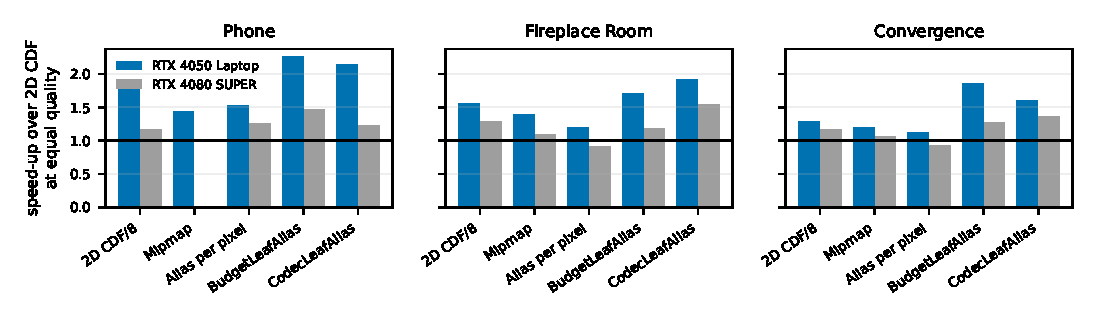
\includegraphics[width=\linewidth]{fig_speedup.pdf}
  \caption{The same numbers as Table~\ref{tab:eq}. Bars above the line are faster than the 2D CDF at
  equal quality. On every scene and for every technique the blue bar is the taller one: the gap to
  the 2D CDF is wider on the smaller processor. Mipmap has no 4080 SUPER bar in Phone because it
  does not reach the 2D CDF's quality there.}
  \label{fig:speedup}
\end{figure}

On the 4080 SUPER the two techniques are between $1.19$ and $1.54$ times faster than the 2D CDF at
equal quality. On the 4050 the same comparison gives $1.60$ to $2.26$. BudgetLeafAlias moves from
$1.47$ to $2.26$ in Phone, $1.19$ to $1.71$ in Fireplace Room and $1.27$ to $1.86$ in Convergence;
CodecLeafAlias from $1.23$ to $2.14$, $1.54$ to $1.92$ and $1.37$ to $1.60$. The ranking is largely
preserved: one of our two is the fastest technique in every scene on both processors, and the two
trade places between scenes on both.

The baselines move in the same direction, which is the part worth stating plainly. The per-pixel
alias table goes from $0.91$ to $1.19$ in Fireplace Room and from $0.93$ to $1.13$ in Convergence,
that is, from slightly slower than the 2D CDF to slightly faster. The trimmed 2D CDF/8 and the
mipmap warp also gain. So the effect is not that our techniques become better on a small GPU; it is
that \emph{the dense 2D CDF becomes worse}, and everything is measured against it. What distinguishes
our two is the size of the gain: BudgetLeafAlias gains $0.52$ to $0.79$ in absolute speed-up where
the per-pixel alias gains $0.20$ to $0.28$.

\begin{figure}[H]
  \centering
  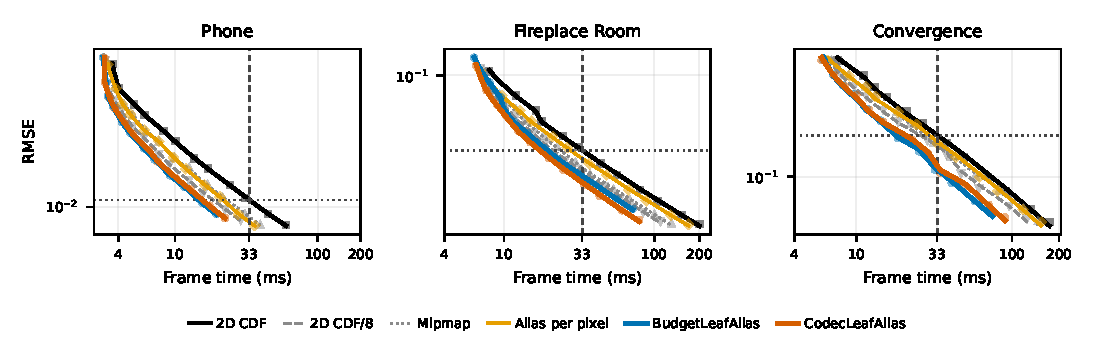
\includegraphics[width=\linewidth]{fig_curves.pdf}
  \caption{RMSE against frame time on the RTX 4050 Laptop (markers: the measured rungs; curves: the
  fits). The vertical line is the 33.3\,ms budget and the horizontal line the RMSE the 2D CDF
  reaches there. A curve lying below and to the left of another is strictly better. Our two
  techniques are the lowest pair across the whole measured range in all three scenes, and the gap
  widens as the budget grows.}
  \label{fig:curves}
\end{figure}

\begin{table}[H]
\centering\small
\setlength{\tabcolsep}{5pt}
\caption{The same 33.3\,ms frame on the RTX 4050 Laptop, read at equal \emph{time} instead of equal quality. \emph{samples}: light samples per shading point that fit in the budget (64 is the engine's limit). \emph{RMSE}: error at that point relative to the 2D CDF's, where below 1 is better.}
\label{tab:op}
\begin{tabular}{l cc cc cc}
\toprule
 & \multicolumn{2}{c}{Phone} & \multicolumn{2}{c}{Fireplace Room} & \multicolumn{2}{c}{Convergence} \\
\cmidrule(lr){2-3}\cmidrule(lr){4-5}\cmidrule(lr){6-7}
Technique & samples & RMSE & samples & RMSE & samples & RMSE \\
\midrule
2D CDF & 34 & 1.000 & 9 & 1.000 & 10 & 1.000 \\
2D CDF/8 & 64 & 0.783 & 17 & 0.794 & 14 & 0.889 \\
Mipmap & 52 & 0.817 & 14 & 0.828 & 13 & 0.907 \\
Alias per pixel & 58 & 0.771 & 11 & 0.916 & 12 & 0.930 \\
\textbf{BudgetLeafAlias} & 64 & 0.847 & 26 & 0.756 & 25 & 0.690 \\
\textbf{CodecLeafAlias} & 64 & 0.809 & 23 & 0.704 & 22 & 0.714 \\
\bottomrule
\end{tabular}
\end{table}


Read at equal time instead (Table~\ref{tab:op}), the picture is the same seen from the other side.
Inside a 33.3\,ms frame on the 4050 the 2D CDF affords 34.5 light samples per shading point in Phone,
8.6 in Fireplace Room and 10.3 in Convergence; BudgetLeafAlias affords 64, 25.9 and 25.2 in the same
budget, and spends those extra samples on 15\%, 24\% and 31\% less error. In Phone both of our
techniques reach the engine's 64-sample limit before the budget is exhausted, finishing the frame in
19.5 and 22.4\,ms against the 2D CDF's 33.3\,ms.

\emph{Why the 2D CDF loses more here.} The explanation is where each structure is read from. The
2D CDF stores one entry per texel, 16.6\,MB for the $1920\times1080$ emitter of Phone and 66\,MB for
the $3840\times2160$ emitters, and performs about 24 dependent reads per sample into it; the
per-pixel alias table stores 41.5\,MB and 166\,MB and performs two. BudgetLeafAlias reads a 75\,KB
table that fits in the 128\,kB first-level cache of \emph{either} processor. The first-level cache is
the same size on both parts, so the cost of our techniques scales with the machine; the per-texel
structures sit in the second-level cache or beyond, and that is the level that shrinks from 64\,MB
to 24\,MB. A dependent read costs 14.4\,ps on this GPU while it hits the first level, 67.7\,ps from
the second, and 530\,ps once it misses both --- a factor of 37 between the two ends.

\section*{4\quad Study 2: the leaf budget}

\begin{table}[H]
\centering\small
\setlength{\tabcolsep}{4pt}
\caption{Leaf budget of BudgetLeafAlias. Left: speed-up over the 2D CDF at equal quality in a 33.3\,ms frame, measured here on the RTX 4050 Laptop. Right: the cost of light sampling alone, relative to that GPU's own $B=1000$, on both GPUs --- the one measurement in this note made with an identical protocol on each. $B=250$ was not run in the sampling benchmark.}
\label{tab:leaves}
\begin{tabular}{l ccc cc cc cc}
\toprule
 & \multicolumn{3}{c}{Speed-up at equal quality (4050)} & \multicolumn{2}{c}{Phone} & \multicolumn{2}{c}{Fireplace Room} & \multicolumn{2}{c}{Convergence} \\
\cmidrule(lr){2-4}\cmidrule(lr){5-6}\cmidrule(lr){7-8}\cmidrule(lr){9-10}
Budget & Phone & Fireplace Room & Convergence & 4050 & 4080S & 4050 & 4080S & 4050 & 4080S \\
\midrule
$B$=250 & -- & 0.88 & 1.60 & -- & -- & -- & -- & -- & -- \\
$B$=1000 & 1.89 & 1.40 & 1.76 & 1.00 & 1.00 & 1.00 & 1.00 & 1.00 & 1.00 \\
$B$=2000 & 2.08 & 1.58 & 1.82 & 1.08 & 1.05 & 0.93 & 1.05 & 1.04 & 1.03 \\
$B$=4000 & 2.26 & 1.71 & 1.86 & 1.19 & 1.16 & 0.88 & 1.15 & 1.08 & 1.12 \\
$B$=8000 & 2.27 & 1.88 & 1.79 & 1.26 & 1.23 & 0.85 & 1.22 & 1.15 & 1.21 \\
$B$=16000 & 2.35 & 1.97 & 1.88 & 1.31 & 1.27 & 0.85 & 1.26 & 1.19 & 1.26 \\
\bottomrule
\end{tabular}
\end{table}


\begin{figure}[H]
  \centering
  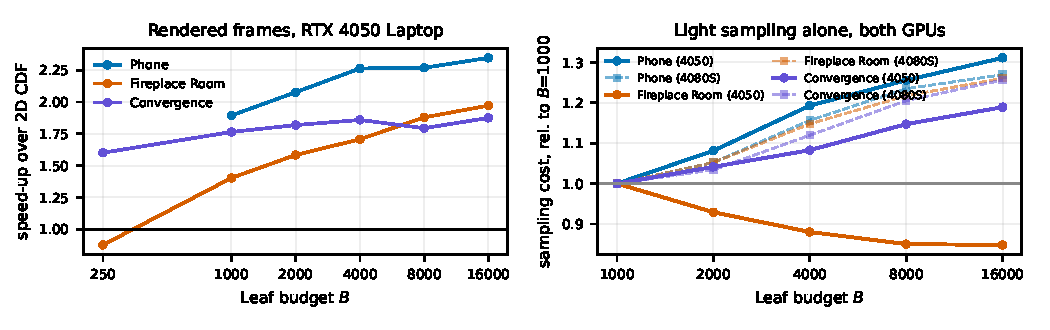
\includegraphics[width=\linewidth]{fig_leaves.pdf}
  \caption{Left: speed-up over the 2D CDF at equal quality in rendered frames on the RTX 4050
  Laptop, against the leaf budget. Right: the cost of light sampling alone, each processor
  normalised to its own $B=1000$ --- the one measurement here made with an identical protocol on
  both parts.}
  \label{fig:leaves}
\end{figure}

The leaf budget $B$ decides how finely BudgetLeafAlias partitions the emitter, and therefore both
how well it matches the light and how large its structure is, at about 19 bytes per leaf: 19\,KB at
$B=1000$, 75\,KB at $B=4000$ and 300\,KB at $B=16000$.

In rendered frames on the 4050 the speed-up rises with $B$ and then flattens. In Phone it goes
$1.89$, $2.08$, $2.26$, $2.27$, $2.35$ for $B$ from 1000 to 16000; in Convergence $1.76$ to $1.88$
across the same range, essentially flat from $B=2000$ on. Fireplace Room is the one scene that keeps
climbing, $1.40$ to $1.97$, because its light is concentrated in a small bright region that a coarse
partition cannot resolve. Below $B=1000$ the technique starts to fail: at $B=250$ it is slower than
the 2D CDF in Fireplace Room ($0.88$) and never reaches the 2D CDF's quality at all in Phone. A
budget of a few thousand leaves is therefore doing real work, and $B=4000$ sits at the point where
the curves have flattened in two scenes out of three.

The right half of Figure~\ref{fig:leaves} is the cost side, and it is the one place in this note
where both processors were measured with the same protocol: an isolated compute dispatch that draws
light samples with no ray tracing or shading, timed with GPU timestamps. From $B=1000$ to
$B=16000$ the cost of sampling rises 31\% in Phone on the 4050 against 27\% on the 4080 SUPER, and
19\% against 26\% in Convergence --- close enough that the structure can be said to behave the same
way on both. Fireplace Room does not: its cost \emph{falls} 15\% on the 4050 where it rises 26\% on
the 4080 SUPER, and the measurement is solid, reproducing to within 0.1\,ms over seven shuffled
rounds. The reason is the same mechanism as above, applied to the texture rather than the structure.
A coarse partition over a $3840\times2160$ emitter whose light sits in one small region spreads the
radiance fetches that follow each sample over a wide area of that texture; a finer partition
concentrates them into a small region that stays in cache. On a part with a quarter of the memory
interface that fetch dominates, and buying a larger structure buys back more than it costs.

The practical reading is that a smaller, cheaper GPU does not want a smaller leaf budget. On this
hardware $B$ between 2000 and 16000 is within a few per cent in cost, the quality it buys is a
property of the partition rather than of the processor, and in the one scene where the two
processors disagree it is the \emph{larger} budget that is cheaper on the smaller part.

\section*{5\quad Scope}

Three scenes were measured. The comparison is of light-sampling performance under
direct illumination, so it says nothing about global illumination, denoising or temporal behaviour.
The 4050 ladders are single frames per rung while the 4080 SUPER equal-quality numbers integrate
over a video, and Section~2 says where that matters. Frame times on the 4050 come from a part whose
clock cannot be locked and which is power limited to 35\,W, so they are medians over forty frames
after a warm-up rather than single readings. Finally, the absolute frame times of the two columns
are not directly comparable and no claim is made from them; every comparison in this note is a ratio
taken within one processor, between a technique and the 2D CDF on that same machine.

\end{document}
